\section{Кинематика дельта-робота}
\subsection{Конструкция и устройство}
Основанием робота является база, жёстко фиксируемая в пространстве над рабочем полем. Габариты базы очерчиваются равносторонним треугольником со стороной равной f. Середины сторон треугольника обозначают координаты осей вращения рычагов и таким образом, расстояние от центра базы до оси вращения каждого рычага равно r - радиусу вписанной окружности равностороннего треугольника. Это расстояние легко находится через соотношение:
\begin{center}
f =$\frac{\sqrt{3}}{2}$  r
\end{center}

Начало координат располагается в центре базы, таким образом, чтобы Z координата высоты равнялась нулю для точек осей вращения рычагов, так как конечное расположение рабочего органа робота будет рассчитываться относительно этих координат. Три рычага нумеруются определённым образом. Первый рычаг двигается в плоскости YZ и направлен в противоположную оси Y сторону. Второй рычаг повернут относительно оси Z на 120 градусов, а третий на -120 градусов. Поворот делается по правилу правой руки, где большой палец совпадает с направлением оси Z, а согнутые пальцы показывают направление вращения. Так как робот в целом абсолютно симметричен, ошибки с нумерацией рычагов закономерны, необходимо на всех этапах строго придерживаться единому правилу обозначения рычагов.

Жёстко закреплённые каждый в своей плоскости рычаги обозначаются $r_{fi}$, а угол на который они поворачиваются обозначают через $\theta_{i}$. Точка оси вращения рычагов обозначается как $F_{i}$, а конечная точка точка рычага - $J_{i}$. На конце рычага находится крепление с двумя карданными шарнирами, которое всегда параллельно стороне равностороннего треугольника, обозначающего габариты рабочего органа. Две взаимно параллельные направляющие соединяются через шарниры с вершинами треугольника, образуя параллелограмм. Из-за этого, данный робот также называют разновидностью параллельного робота.

Для математического описания робота карданные шарниры и параллельные направляющие не нужны, их заменяют рычагами обозначаемыми как $r_{ei}$. Рычаги $r_{ei}$ крепятся к серединам сторон треугольника, обозначающего габариты рабочего органа. Длина стороны обозначается буквой e. Координаты точек крепления называют $E_{i}$, а точкой $E_{0}$ обозначается координата рабочего органа.
\begin{figure}[h!]
	\centering
	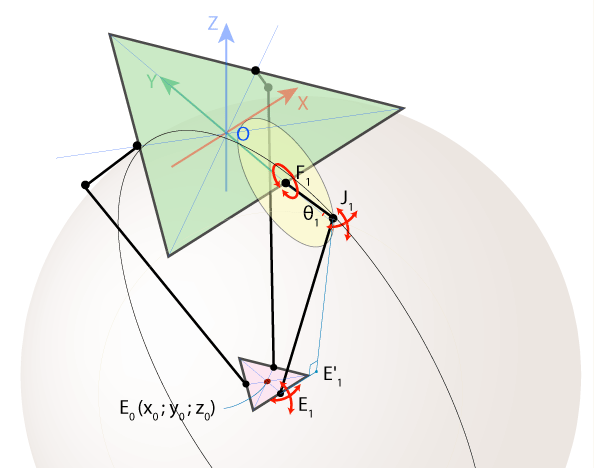
\includegraphics[width=0.8\linewidth]{image/deltabot}
	\caption{Схематическое представление Дельта-робота}
	\label{fig:TotalConsumption}
\end{figure}




\subsection{Прямая}
\subsection{Обратная}

